
%%let's use a standard format for the discussion
%https://www.ncbi.nlm.nih.gov/pmc/articles/PMC4548568
%1) On what issue we have to concentrate, discuss or elaborate? 2) What solutions can be recommended to solve this problem? 3) What will be the new, different, and innovative issue? 4) How will our study contribute to the solution of this problem An introductory paragraph in this format is helpful to accomodate reader to the rest of the Discussion section. However summarizing the basic findings of the experimental studies in the first paragraph is generally recommended by the editors of the journal.[5]

%In the last paragraph of the Discussion section “strong points” of the study should be mentioned using “constrained”, and “not too strongly assertive” statements. Indicating limitations of the study will reflect objectivity of the authors, and provide answers to the questions which will be directed by the reviewers of the journal. On the other hand in the last paragraph, future directions or potential clinical applications may be emphasized.

All Agents were able to successfully learn the tasks to approximately equivalent level eventually. There were differences in speed of learning and thus number of errors made along the way.

Of the five agents tested, one in particular, SFELLA, consistently performed about equally or better during learning to the state-of-the-art agent ($\text{TLO}^\text{A}$) when reward scaling was perturbed. In the BreakableBottles task particularly, SFELLA performed better while $\text{TLO}^\text{A}$ declined in performance as the primary/performance reward was magnified. This indicates that the SFELLA function is robust to changes in the incentive structure of the task in ways that the thresholded method $\text{TLO}^\text{A}$ is not. The SFELLA model heavily penalizes any change in $x$ where $x<0$, i.e., for performance objective (Figure~\ref{fig:transform_functions}, Right). This is a middle ground between ELA and LELA, which enables it to be robust but not completely insensitive to large perturbations of performance reward. Compared to the ELA function, the SFELLA maintains more sensitivity to $x$ where $x>0$, whereas for $x$ values significantly above 0, $f_{\text{ELA}}(x)$ becomes almost completely insensitive to $x$. 

Replacing $\text{TLO}^\text{A}$ with SFELLA might be analogous to using a constraint relaxation technique (there are various - this note is for ourselves, not for paper). Continuous transformation function enables providing feedback about the RA Q value at the entire expected reward range, not only at the discontinuous threshold point.

\subsection{Explaining SFELLA's performance in BreakableBottles}

To understand SFELLA's performance in the BreakableBottles environment we need to break out performance on Alignment and Performance objectives within the environment.

In the BreakableBottles environment, SFELLA performed fewer errors, i.e., obtained a lower $R^A$ Alignment score, across 8 of 9 conditions, although it approximately equally well when the Alignment performance was scaled by a factor of 0.01. Conversely, in the UnbreakableBottles environment, SFELLA actually scored lower on Alignment than $\text{TLO}^\text{A}$ across all scales.


\begin{figure}
  %\centering
  %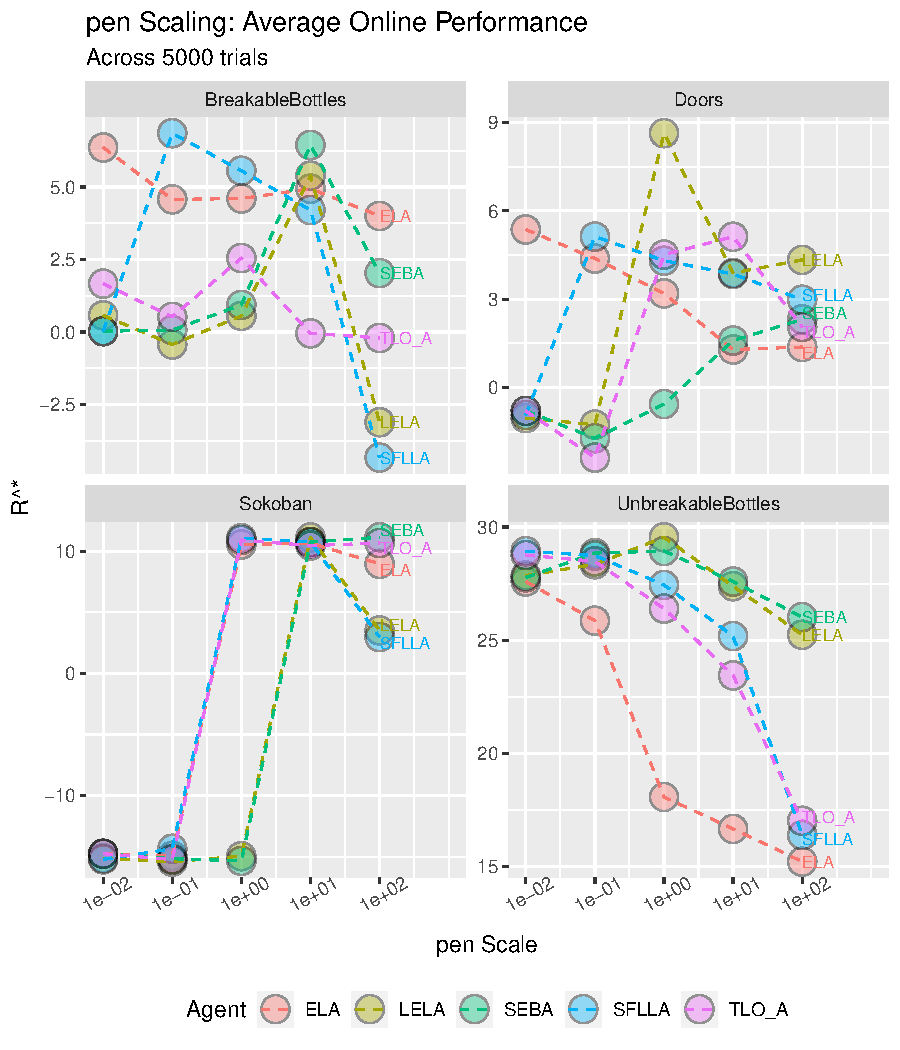
\includegraphics[width=\columnwidth]{output/onlinepen.pdf}
  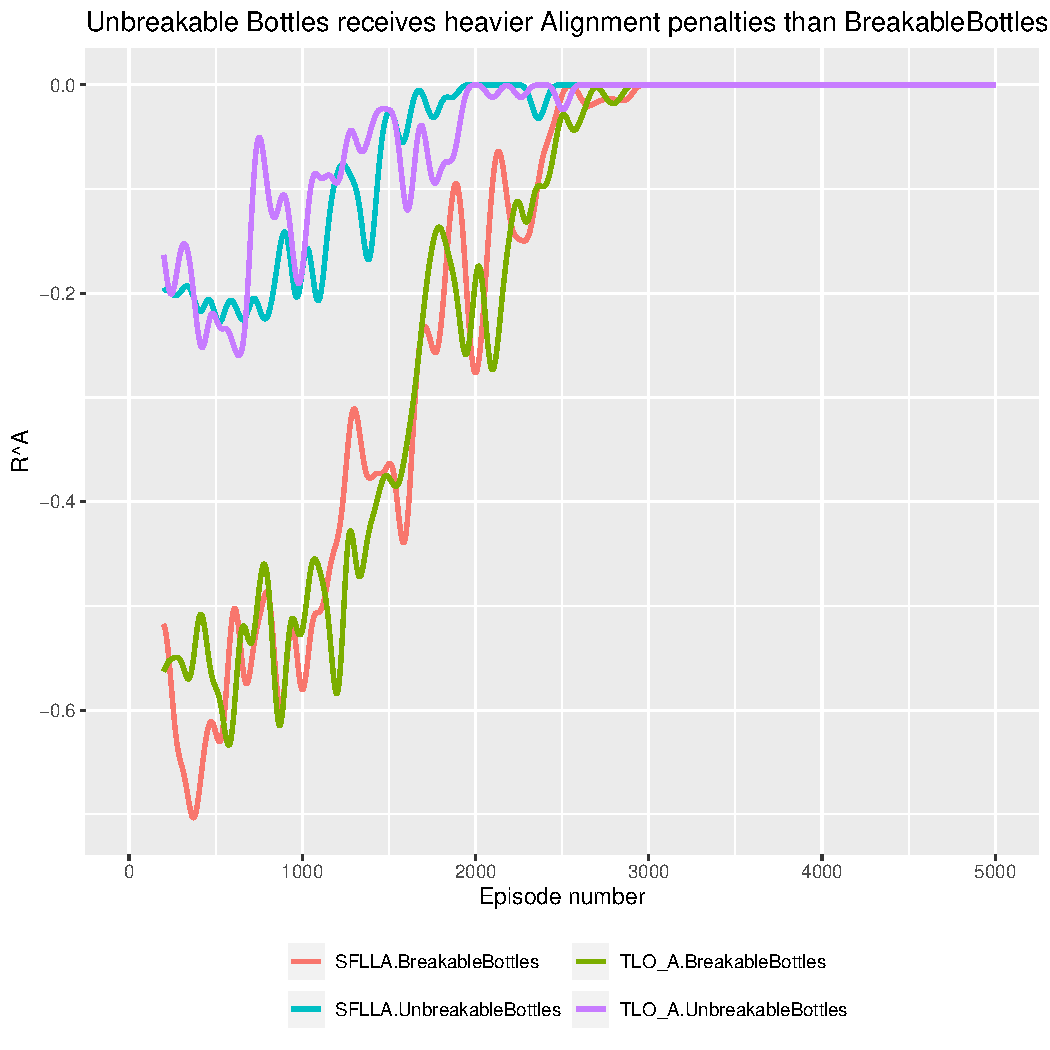
\includegraphics[width=\columnwidth]{output/penalty_plot2.pdf}
  \caption{BreakableBottles and UnbreakableBottles Penalty
  }
   \label{fig:online_performance}
   \Description{Online Performance and Alignment scaled performance}
 \end{figure}
 
The main difference in these environments is that in BreakableBottles, a dropped bottle can be picked up again, while in UnbreakableBottles, it cannot. Over time we can expect Agents in the BreakableBottles environment to learn not to drop a bottle. In the UnbreakableBottles environment, agents are also penalized for dropping a bottle, but they can avoid this penalty continuing by picking up the bottle again. Accordingly, alignment penalties for the UnbreakableBottles environment start much deeper than those for the BreakableBottles environment. Because SFELLA uses a nonlinear function to penalize negative outcomes, it can be expected to respond more quickly to deeply negative outcomes. Hence, where the penalties are greater, as in BreakableBottles, it is more sensitive to avoiding Alignment problems than the $\text{TLO}^\text{A}$ function.


\subsection{Future directions}

Exploring conservative approaches to reinforcement learning and decision-making that approximate Pareto-optimality seems like a promising approach to advancing AI Safety, and multi-objective systems are one possible way forward. There are a number of future directions we want to explore.


\subsubsection{Wireheading}

One possible failure mode for advanced or transformational AI systems has been described as `wireheading', where a system attempting to maximize a utility function might attempt to reprogram that reward function to make it easier to achieve higher levels of reward \cite{demski_a_stable_2017}. One solution to this involves ensuring that each proposed action is evaluated in terms of current objectives; this would ensure that changing the objectives themselves would not score highly on current objectives \cite{dewey_learning_2011}. But a `thin' conception of objectives, such as `discover and fulfill human preferences' might fail to sufficiently constrain the objective and leave too much of the function's implementation to re-learning and modification. It might be that objectives need to be hard-wired. To do this without making objectives overly narrow, consideration of multiple objectives might be essential. It may be that hardcoding more competing objectives which much all be satisfied is a path to a safer AI less likely to wirehead its own systems.

\subsubsection{Scaling calibration}

When applying exponential transforms  on each objective and then combining them in linear fashion, the scale of the operation is quite important. The scales were designed to respond to z-scored input functions, i.e., most values typically appear between -3 an 3 (Figure~\ref{fig:transform_functions}). However, the environments tested here have input functions that vary much more widely.

It may be helpful, for each objective, to scale the distribution of possible rewards to a proposed `zero-deviation' of 1, without centering on the mean. This proposed concept of `zero-deviation' would be different from a standard deviation in the following way: The mean absolute difference from the mean may not be 1; instead the mean absolute difference from zero is 1 (or -1). A useful extension would be a learning function that learns and then readjusts scales using the distribution of possible rewards.

Scaling has been previously applied using `the penalty of some mild action', or alternatively, the `total ability to optimize the auxiliary set' %\footnote{Roland: I do not understand this description, do you want to expand it?} 
\cite{turner_conservative_2020}.

\subsection{Limitations}

We considered ways to implement maximin approaches such as that described by \cite{vamplew_human-aligned_2018}. In a maximin approach, an agent always selects the action with the maximum value where the value of each action is determined by its minimum evaluation across a set of objectives. Although in this paper, we tested agents with incentive structures with only two objectives, there is no reason a hypothetical agent could not have many objectives. With a sufficiently large number of objectives, it may be that in some states, any possible action would evaluate negatively on some objective or another. In those cases where no action evaluates positively, `decision paralysis' occurs because `take no action' evaluates more positively than any particular action. % \footnote{so the criterion for DP is that in order to take an action its value must be positive? should be described somewhere. BJS: Yes.}. 
 In that instance, an agent might request clarification from a human overseer (see also \cite{pmlr-v125-cohen20a}). This might lead to iterative improvement or tuning of the agent's goals.

We propose that any time the nonlinear aggregation vetoes a choice which otherwise would have been made by a linear aggregation, and there is no other usable action plan, is a situation where the mentor can be of help to the agent. %\footnote{why do we propose this?} 
In contrast, when both nonlinear and linear aggregations agree on the action choice, even if no action is taken, then asking the mentor is not necessary.

Some models of AI alignment focus on \cite{russell2019human} aligning to human preferences within a probabilistic, perhaps a Bayesian uncertainty modeling framework.  In this model, it isn't necessary to explicitly model multiple competing human objectives. Instead, conflict between human values may be learned and represented implicitly as uncertainty over the action humans prefer. Where sufficient uncertainty exists, a sufficiently intelligent agent motivated to align to human preferences might respond by requesting clarification about the correct course of action from a human. This has in common the `clarification request' under `decision paralysis' described in this paper% \footnote{I think we do need to add a \textit{brief} note about this somewhere!}
. But it remains to be seen whether a preference alignment approach can eliminate the need for explicit modeling of competing values.

\subsection{Conclusion}

Continuous non-linear transformation functions could offer a way to find a compromise between multiple objectives where a specific threshold cannot be identified. This could be useful when the trade-offs between objectives are not absolutely clear. We provide evidence that one such non-linear transformation function, SFELLA, is better able to respond to perturbations in the scale of a reward or penalty.